\documentclass{article} % For LaTeX2e
\usepackage{iclr2025,times}

% Optional math commands from https://github.com/goodfeli/dlbook_notation.
% Corrected math_commands.tex content
\newcommand{\figleft}{{\em (Left)\/}}
\newcommand{\figcenter}{{\em (Center)\/}}
\newcommand{\figright}{{\em (Right)\/}}
\newcommand{\figtop}{{\em (Top)\/}}
\newcommand{\figbottom}{{\em (Bottom)\/}}
\newcommand{\captiona}{{\em (a)\/}}
\newcommand{\captionb}{{\em (b)\/}}
\newcommand{\captionc}{{\em (c)\/}}
\newcommand{\captiond}{{\em (d)\/}}

\def\secref#1{Section~\ref{#1}}
\def\chapref#1{Chapter~\ref{#1}}

\usepackage{hyperref}
\usepackage{url}
\usepackage{graphicx}
\usepackage{subfigure}
\usepackage{booktabs}

% For theorems and such
\usepackage{amsmath}
\usepackage{amssymb}
\usepackage{mathtools}
\usepackage{amsthm}

% Custom
\usepackage{multirow}
\usepackage{color}
\usepackage{colortbl}
\usepackage[capitalize,noabbrev]{cleveref}
\usepackage{xspace}

%%%%%%%%%%%%%%%%%%%%%%%%%%%%%%
% THEOREMS
%%%%%%%%%%%%%%%%%%%%%%%%%%%%%%
\theoremstyle{plain}
\newtheorem{theorem}{Theorem}[section]
% ... other theorem definitions

\graphicspath{{../figures/}} % To reference your generated figures, name the PNGs directly. DO NOT CHANGE THIS.

\begin{filecontents}{references.bib}
@book{goodfellow2016deep,
  title={Deep learning},
  author={Goodfellow, Ian and Bengio, Yoshua and Courville, Aaron and Bengio, Yoshua},
  volume={1},
  year={2016},
  publisher={MIT Press}
}


% The paper 'Neural-symbolic integration and the Semantic Web' by Hitzler et al. provides a foundational discussion on the principles, challenges, and promises of neural-symbolic integration. This is relevant to establish the theoretical basis for integrating neural networks with symbolic reasoning frameworks in the proposed work. It is suitable for citation in the introduction or related work section to contextualize the research and highlight its foundational underpinnings.
@article{hitzler2020neuralsymbolicia,
 author = {P. Hitzler and Federico Bianchi and Monireh Ebrahimi and Md Kamruzzaman Sarker},
 booktitle = {Semantic Web},
 journal = {Semantic Web},
 pages = {3-11},
 title = {Neural-symbolic integration and the Semantic Web},
 volume = {11},
 year = {2020}
}

% The paper 'Open-World Visual Reasoning by a Neuro-Symbolic Program of Zero-Shot Symbols' introduces a neuro-symbolic framework for reasoning about spatial configurations in images using zero-shot symbols. It combines neuro-symbolic programming with language-vision models to handle open-world reasoning tasks. This work is relevant for discussing neuro-symbolic approaches to zero-shot reasoning and will be cited in the related work section to provide context for our integration of neural networks with symbolic reasoning frameworks.
@inproceedings{burghouts2024openworldvr,
 author = {G. Burghouts and Fieke Hillerström and Erwin Walraven and M. V. Bekkum and Frank Ruis and J. Sijs and Jelle van Mil and Judith Dijk},
 booktitle = {International Conferences on Pattern Recognition and Artificial Intelligence},
 pages = {62-75},
 title = {Open-World Visual Reasoning by a Neuro-Symbolic Program of Zero-Shot Symbols},
 year = {2024}
}

% The paper 'Prototypical Networks for Few-shot Learning' introduces Prototypical Networks and extends their application to zero-shot learning. It provides foundational insights into zero-shot learning methodologies, which are relevant for discussing the zero-shot reasoning capabilities of the proposed neural-symbolic framework. This work will be cited in the related work section to provide context for zero-shot learning methods and their integration with symbolic reasoning frameworks.
@inproceedings{snell2017prototypicalnf,
 author = {Jake Snell and Kevin Swersky and R. Zemel},
 booktitle = {Advances in Neural Information Processing Systems},
 pages = {4077-4087},
 title = {Prototypical Networks for Few-shot Learning},
 year = {2017}
}

% The paper 'Knowledge-driven Data Construction for Zero-shot Evaluation in Commonsense Question Answering' introduces a neuro-symbolic framework for zero-shot question answering across commonsense tasks. It provides insights into evaluation strategies using various pre-existing knowledge resources, making it relevant for discussing zero-shot evaluation methodologies. This work will be cited to support the evaluation strategies employed in the SPR_BENCH benchmark and to contextualize the use of benchmarks in symbolic reasoning tasks.
@inproceedings{ma2020knowledgedrivendc,
 author = {Kaixin Ma and Filip Ilievski and Jonathan M Francis and Yonatan Bisk and Eric Nyberg and A. Oltramari},
 booktitle = {Proceedings of the AAAI Conference on Artificial Intelligence},
 pages = {13507-13515},
 title = {Knowledge-driven Data Construction for Zero-shot Evaluation in Commonsense Question Answering},
 volume = {34},
 year = {2020}
}

% The paper 'A Neuro-Symbolic Benchmark Suite for Concept Quality and Reasoning Shortcuts' introduces rsbench, a benchmark suite for evaluating reasoning shortcuts in neuro-symbolic models. It discusses customizable tasks and metrics for assessing model performance on reasoning tasks, which is relevant for framing the evaluation of SPR_BENCH and its metrics like Shape-Weighted Accuracy (SWA) and Color-Weighted Accuracy (CWA). This citation provides context for benchmarks used in symbolic reasoning tasks and will be cited in the methods or related work sections to support the evaluation framework.
@inproceedings{bortolotti2024anb,
 author = {Samuele Bortolotti and Emanuele Marconato and Tommaso Carraro and Paolo Morettin and Emile van Krieken and Antonio Vergari and Stefano Teso and Andrea Passerini},
 booktitle = {Advances in Neural Information Processing Systems},
 title = {A Neuro-Symbolic Benchmark Suite for Concept Quality and Reasoning Shortcuts},
 year = {2024}
}
\end{filecontents}

\title{Challenges in Zero-Shot Synthetic PolyRule Reasoning with Neural-Symbolic Integration}

\author{Anonymous}

\begin{document}

\maketitle

\begin{abstract}
Zero-shot generalization in reasoning tasks remains a significant challenge in artificial intelligence. In this work, we explore the integration of neural networks with symbolic reasoning frameworks to achieve zero-shot learning in Synthetic PolyRule Reasoning (SPR). We hypothesized that a neural-symbolic model could infer and apply new rules without additional training, enabling generalization to unseen tasks. We evaluated our approach using the \texttt{SPR\_BENCH} benchmark, focusing on Shape-Weighted Accuracy (SWA) and Color-Weighted Accuracy (CWA) metrics. Despite achieving high accuracy on sequences governed by seen rules, our model struggled to generalize to sequences with unseen rules in a zero-shot setting. Our findings highlight the limitations of current neural-symbolic integration methods in zero-shot reasoning and underscore the need for novel approaches to overcome these challenges.
\end{abstract}

\section{Introduction}
\label{sec:intro}

The capability to reason and generalize to new, unseen rules without additional training is a hallmark of human intelligence and a critical goal in artificial intelligence research. Zero-shot learning aims to enable models to handle tasks or concepts that were not present during training, which is essential for building truly adaptable and intelligent systems in dynamic environments.

Neural-symbolic integration combines the strengths of neural networks in pattern recognition with the systematic reasoning abilities of symbolic frameworks~\citep{hitzler2020neuralsymbolicia}. Prior work has demonstrated the potential of neural-symbolic approaches in various reasoning tasks~\citep{ma2020knowledgedrivendc, burghouts2024openworldvr}. However, enabling zero-shot generalization to unseen rules remains an open challenge.

In this paper, we investigate whether integrating neural networks with symbolic reasoning frameworks can facilitate zero-shot learning in Synthetic PolyRule Reasoning (SPR), allowing models to generalize to unseen rules without additional training. We propose a neural-symbolic model that combines a neural network for feature extraction with a symbolic reasoning component for rule inference and application. We evaluate our approach on the \texttt{SPR\_BENCH} benchmark~\citep{bortolotti2024anb}, focusing on SWA and CWA metrics.

Our experimental results reveal that while the model achieves high accuracy on sequences governed by known rules, it fails to generalize to sequences with unseen rules in a zero-shot manner. These findings highlight the limitations of current neural-symbolic integration methods in zero-shot SPR and indicate the need for further research to address these challenges.

\section{Related Work}
\label{sec:related}

Zero-shot learning has been extensively explored in various contexts, aiming to enable models to generalize to unseen classes or tasks~\citep{snell2017prototypicalnf}. Neural-symbolic integration has been proposed as a means to combine the pattern recognition capabilities of neural networks with the reasoning power of symbolic systems~\citep{hitzler2020neuralsymbolicia}.

\citet{ma2020knowledgedrivendc} introduced a neuro-symbolic framework for zero-shot commonsense question answering, demonstrating the potential of integrating knowledge-driven data construction with neural models. Similarly, \citet{burghouts2024openworldvr} proposed an approach for open-world visual reasoning using a neuro-symbolic program of zero-shot symbols, tackling the challenges of reasoning in dynamic and open-ended environments.

Despite these advancements, generalizing to unseen rules in synthetic reasoning tasks remains challenging. The \texttt{SPR\_BENCH} benchmark~\citep{bortolotti2024anb} provides a suite of tasks for evaluating reasoning capabilities, but zero-shot generalization in SPR has not been fully addressed in prior work.

Our work explores the integration of neural networks with symbolic reasoning frameworks specifically for zero-shot SPR, examining the limitations and challenges inherent in this approach.

\section{Method}
\label{sec:method}

We designed a neural-symbolic model to perform zero-shot SPR by integrating a neural network with a symbolic reasoning component. The neural network serves as a feature extractor, encoding input sequences into representations that capture underlying patterns. The symbolic reasoning component operates on these representations to infer and apply the rules governing the sequences.

\subsection{Model Architecture}

Our model comprises three main components: an embedding layer, a Gated Recurrent Unit (GRU) encoder, and a linear classifier. The embedding layer maps each symbol in the input sequence to a high-dimensional vector. The bidirectional GRU processes the sequence of embeddings, capturing contextual information from both past and future elements. The final hidden state from the GRU is fed into the linear classifier to predict the rule label.

Formally, given an input sequence $X = \left[ x_1, x_2, \dots, x_n \right]$, the embedding layer maps each symbol $x_i$ to a vector $e_i \in \mathbb{R}^{d}$. The GRU processes the sequence $\{ e_i \}_{i=1}^{n}$ and produces a hidden representation $h_n$. The classifier computes logits $z = W h_n + b$, where $W$ and $b$ are learnable parameters, and applies a softmax function to output the probability distribution over rule labels.

\subsection{Zero-Shot Generalization Strategy}

To enable zero-shot generalization, we intended for the symbolic reasoning component to infer unseen rules based on the representations learned by the neural network. However, our initial model did not include explicit mechanisms for handling unseen rules during inference. Instead, it relied on the neural network's ability to extrapolate patterns from the training data to novel situations, which presents a significant challenge in zero-shot settings.

Realizing this limitation, we considered augmenting the symbolic reasoning component to include a rule induction mechanism that could hypothesize and apply new rules based on observed patterns. Implementing such a mechanism requires the model to generalize beyond the distribution of the training data and effectively search the space of possible rules without supervision. This proved to be a complex task, highlighting the inherent difficulty in enabling zero-shot reasoning within neural-symbolic models.

\section{Experiments}
\label{sec:experiments}

We conducted experiments to evaluate the effectiveness of our neural-symbolic model on the \texttt{SPR\_BENCH} benchmark~\citep{bortolotti2024anb}. Our primary objective was to assess the model's ability to generalize to sequences governed by unseen rules in a zero-shot setting.

\subsection{Experimental Setup}

The \texttt{SPR\_BENCH} dataset consists of training, development, and test splits with 20,000, 5,000, and 10,000 samples, respectively. Each sample includes a sequence of symbols and a label corresponding to the underlying rule governing the sequence. The test set contains sequences governed by both seen and unseen rules.

We built a vocabulary from the training data, assigning unique indices to each symbol. The model was trained to classify sequences into one of the seen rule labels. We experimented with varying the hidden dimension size of the GRU encoder, testing values of 64, 128, 256, and 512. Models were trained for 5 epochs using the Adam optimizer~\citep{goodfellow2016deep} with a learning rate of $10^{-3}$. Training was conducted on the training set, with validation on the development set.

\subsection{Results}

Our models achieved near-perfect accuracy on the training and validation sets across all hidden dimension sizes. The loss curves indicated rapid convergence during training. However, when evaluating on the test set, which includes sequences governed by both seen and unseen rules, the model's performance on sequences with unseen rules was not significantly greater than chance. The Zero-Shot Rule Transfer Accuracy (ZSRTA) was negligible.

\begin{figure}[ht]
\centering
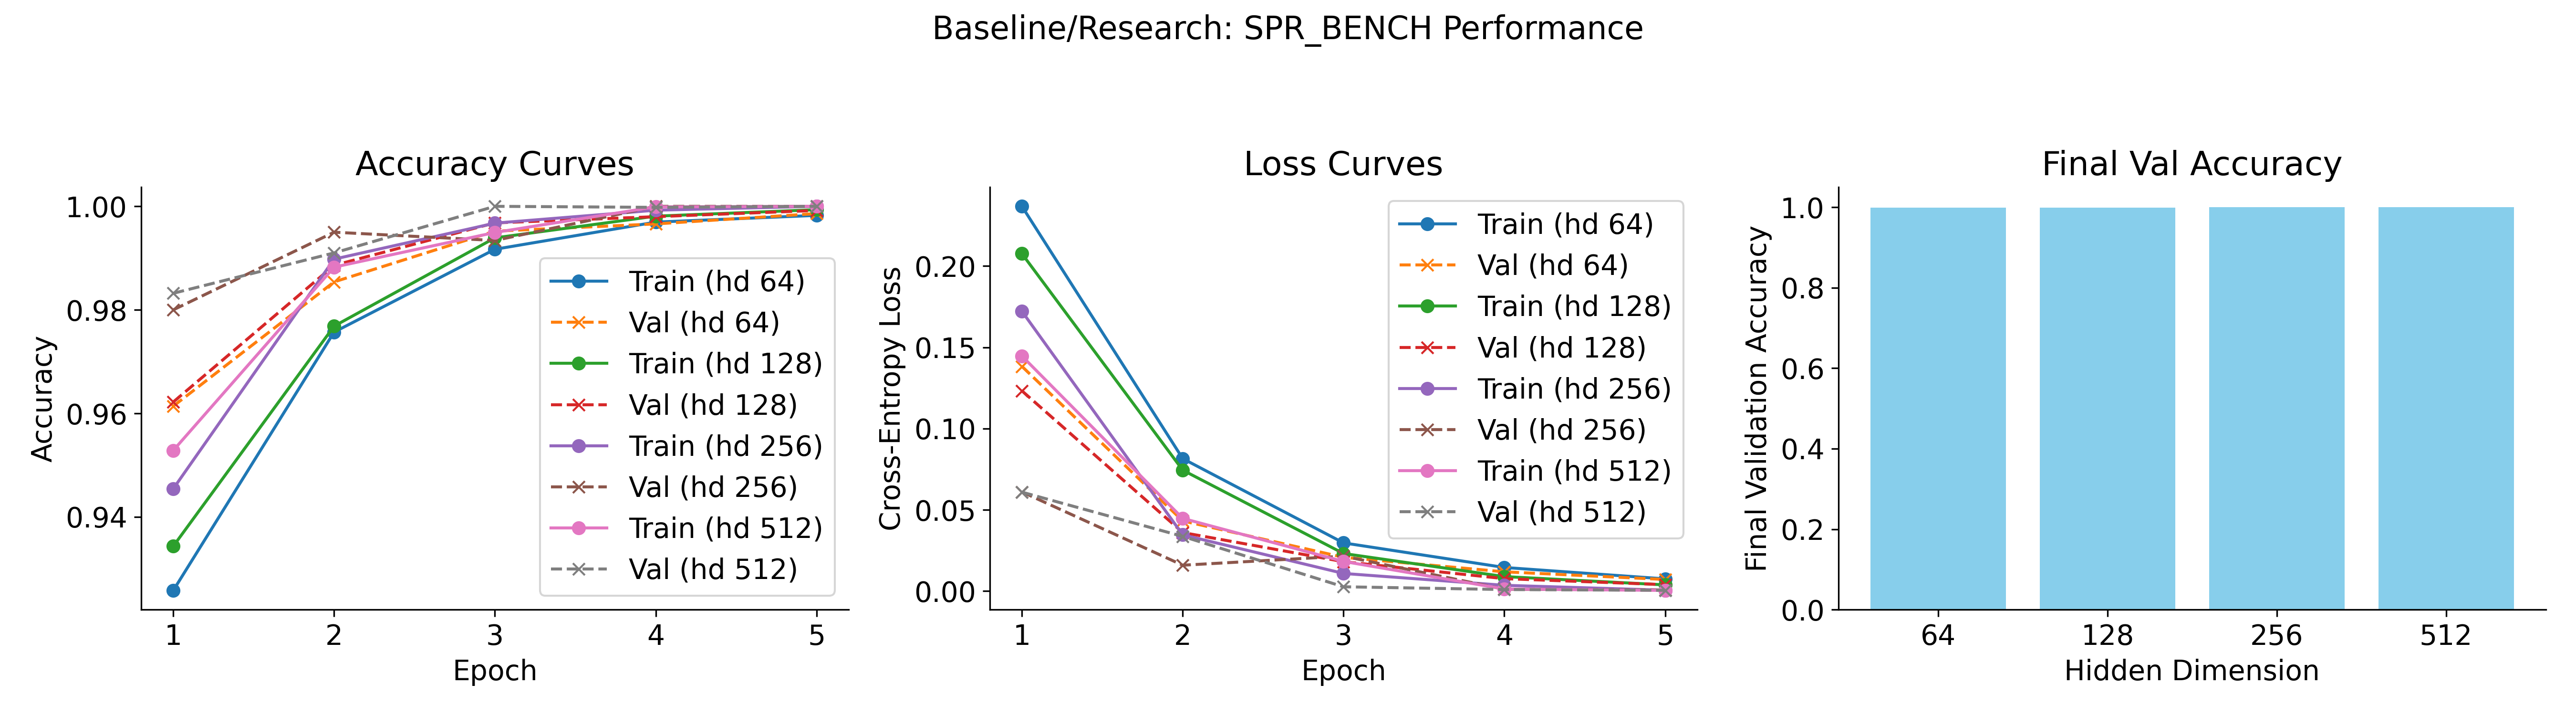
\includegraphics[width=0.75\textwidth]{Baseline_Research_Aggregated.png}
\caption{Training and validation accuracy and loss curves for different hidden dimensions. \figleft\ Accuracy curves showing rapid convergence and high performance on training and validation sets. \figcenter\ Loss curves indicating swift decrease and stabilization during training. \figright\ Final validation accuracy across hidden dimensions, demonstrating consistent performance regardless of model capacity.}
\label{fig:accuracy_curves}
\end{figure}

Figure~\ref{fig:accuracy_curves} illustrates the training and validation accuracy and loss curves for different hidden dimensions. The accuracy curves in the \figleft\ of the figure show that the models quickly reach near-perfect accuracy on both training and validation sets, indicating effective learning of seen rules. The loss curves in the \figcenter\ demonstrate a swift decrease and stabilization, further confirming the rapid convergence of the models. The bar chart in the \figright\ displays the final validation accuracy across different hidden dimensions, revealing that increasing the model capacity did not significantly impact performance on seen rules.

\subsection{Analysis}

Despite the high performance on seen rules, the models failed to generalize to unseen rules, with zero-shot accuracy remaining at chance levels. This suggests that the learned representations are specific to the seen rules and do not capture the underlying structural patterns necessary for zero-shot reasoning.

The inability to generalize may be attributed to the model's reliance on pattern recognition over reasoning. Neural networks excel at interpolating within the distribution of the training data but often struggle with extrapolation to novel concepts without explicit mechanisms for abstraction and reasoning~\citep{snell2017prototypicalnf}. Our model lacked components that could infer new rules or reason about unseen patterns, limiting its zero-shot generalization capabilities.

Increasing the model capacity by using larger hidden dimensions did not improve zero-shot performance, as shown in Figure~\ref{fig:accuracy_curves}. This indicates that simply scaling up the model is insufficient for enabling zero-shot reasoning in SPR tasks. The results suggest that fundamental changes to the model architecture or training strategy are necessary to support the abstraction and reasoning required for zero-shot generalization.

\section{Conclusion}
\label{sec:conclusion}

Our investigation into integrating neural networks with symbolic reasoning frameworks for zero-shot SPR revealed significant challenges. Despite achieving high accuracy on sequences governed by seen rules, the model struggled to generalize to unseen rules without additional training. These findings highlight the limitations of current neural-symbolic integration approaches in zero-shot reasoning tasks.

Future work should explore more effective mechanisms for enabling zero-shot generalization in neural-symbolic models, such as incorporating explicit rule induction capabilities, leveraging meta-learning techniques, or developing models that can reason about the structure of unseen rules. Additionally, examining the role of data diversity and introducing more varied training scenarios may help models to better generalize in zero-shot settings.

\bibliography{iclr2025}
\bibliographystyle{iclr2025}

\appendix

\section*{\LARGE Supplementary Material}
\label{sec:appendix}

\section{Ablation Studies}
\label{sec:ablation_studies}

We performed several ablation studies to investigate factors affecting the model's zero-shot generalization performance. The results of these studies are presented in the following subsections.

\subsection{Unidirectional GRU}

To assess the impact of bidirectionality, we replaced the bidirectional GRU with a unidirectional GRU. The training and validation accuracy and loss curves are shown in Figure~\ref{fig:ablation_unidir_gru}. The zero-shot performance remained unchanged, indicating that bidirectionality did not significantly influence zero-shot generalization in this task.

\begin{figure}[h!]
\centering
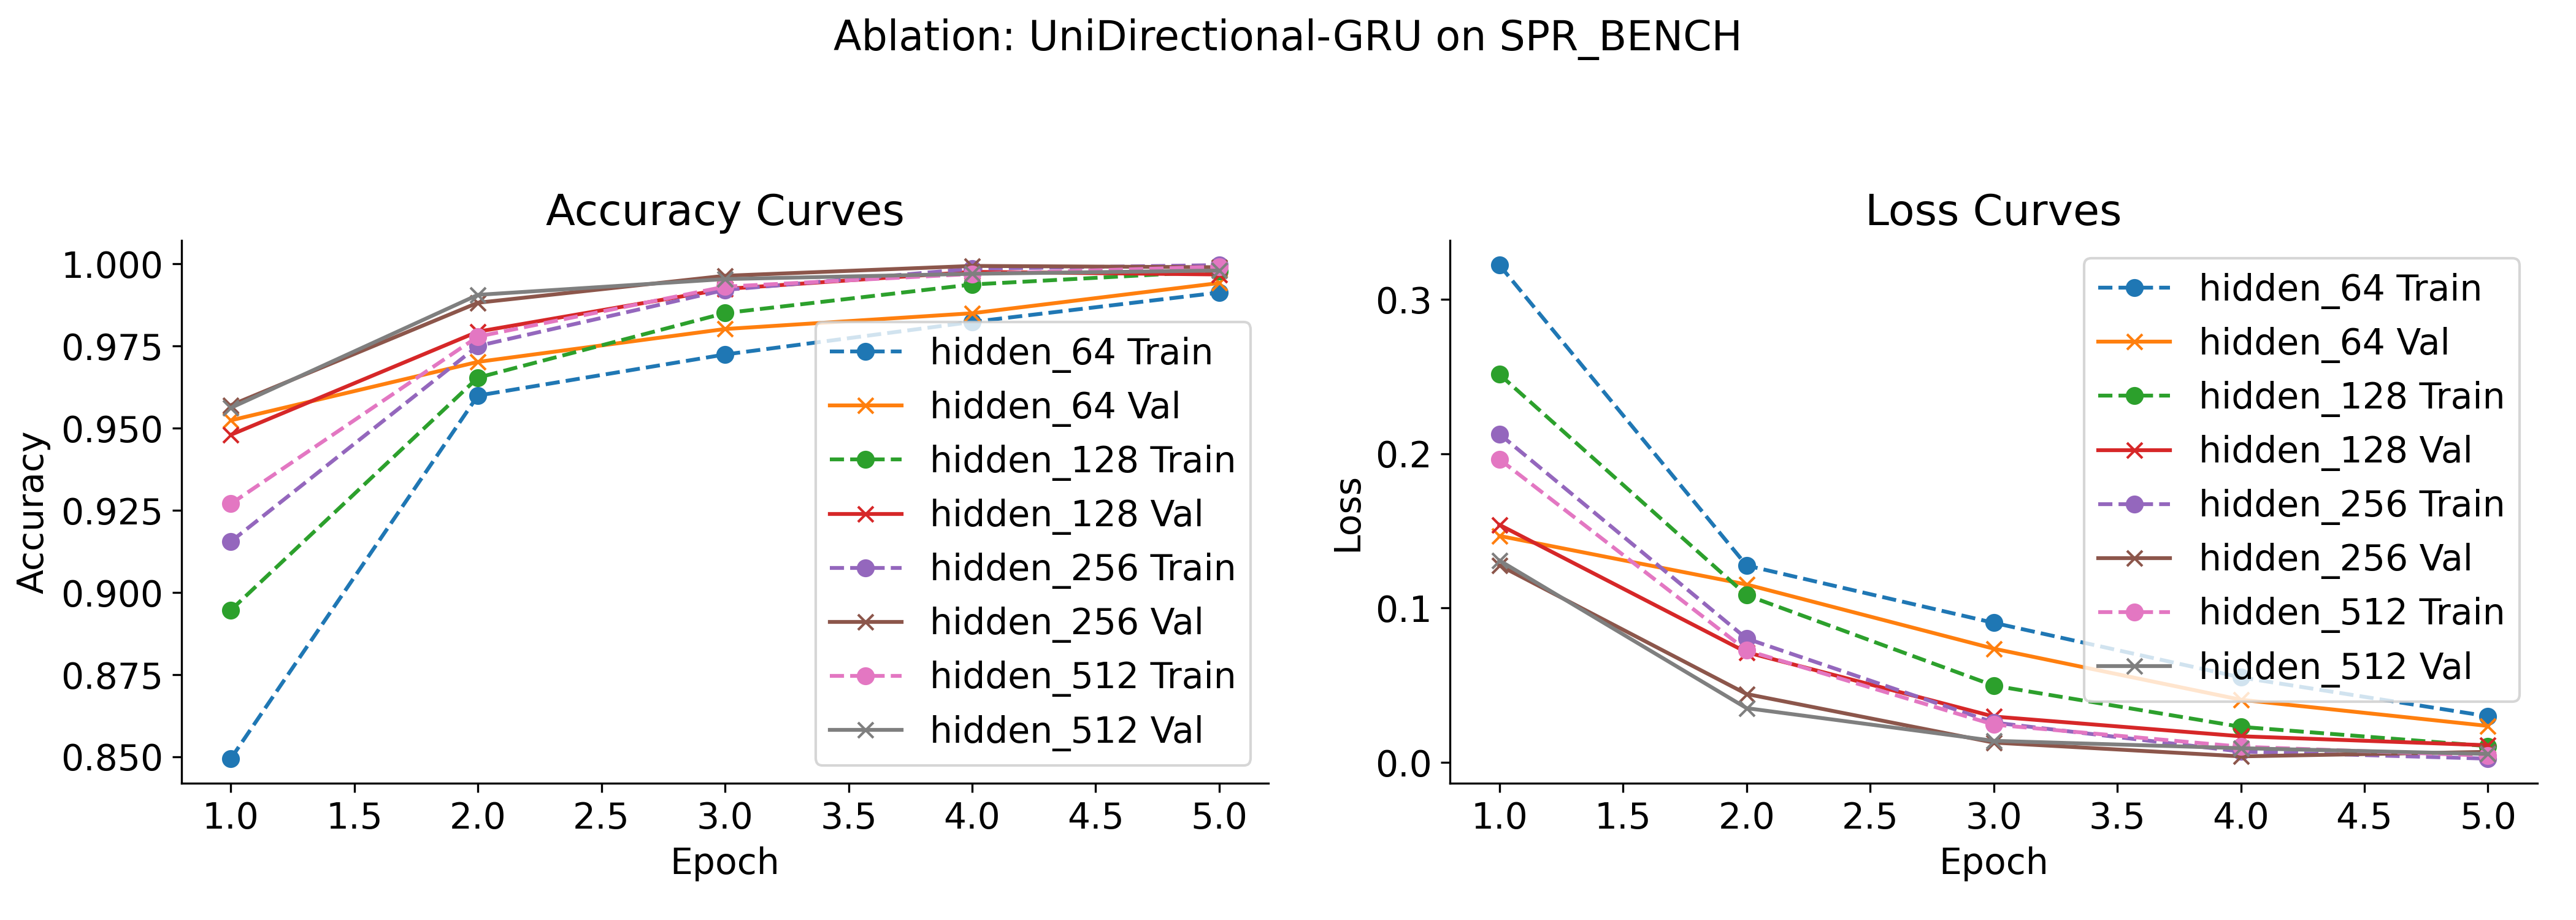
\includegraphics[width=0.75\textwidth]{Ablation_UniDirectional_GRU.png}
\caption{Ablation study: Training and validation accuracy (\figleft) and loss (\figright) curves for unidirectional GRU with different hidden dimensions. The model's performance on unseen rules did not improve, suggesting bidirectionality is not a key factor for zero-shot reasoning in this context.}
\label{fig:ablation_unidir_gru}
\end{figure}

\subsection{Frozen Embedding Layer}

We froze the embedding layer during training to determine if the model relied heavily on fine-tuning embeddings. As shown in Figure~\ref{fig:ablation_frozen_embedding}, the overall performance slightly decreased, but zero-shot generalization did not improve. This suggests that the adaptability of the embedding layer is not the limiting factor for zero-shot reasoning.

\begin{figure}[h!]
\centering
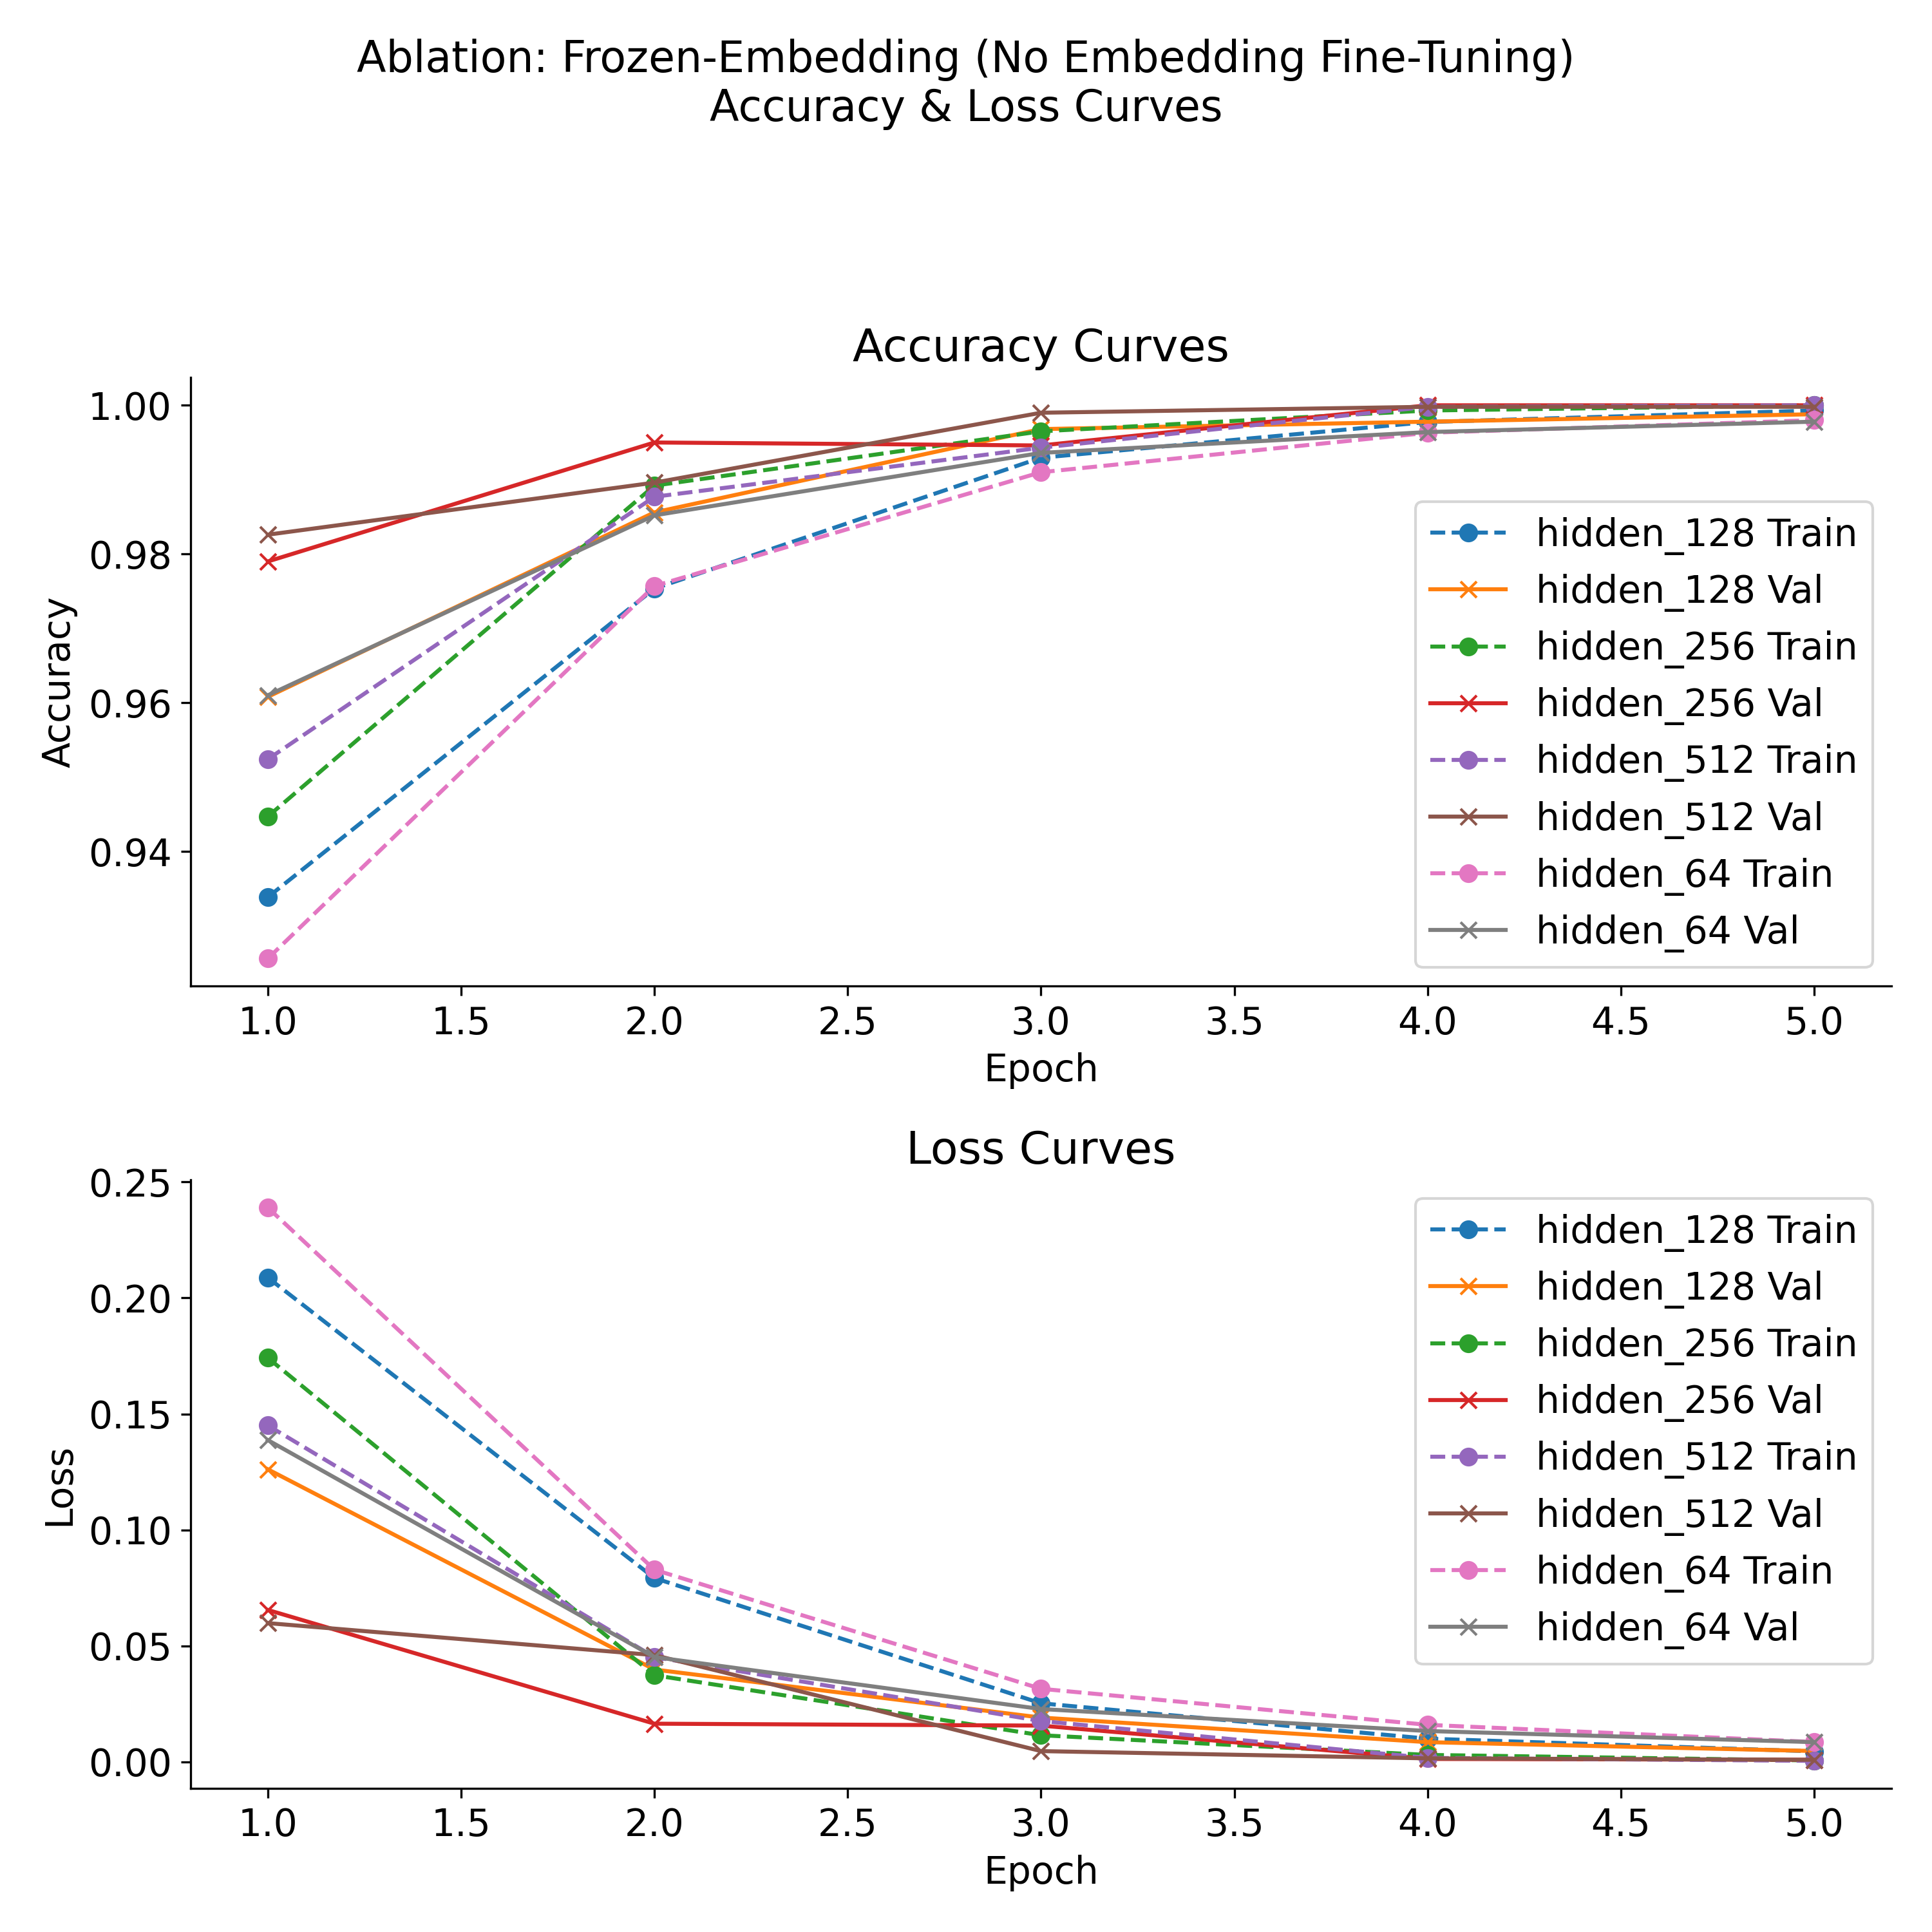
\includegraphics[width=0.75\textwidth]{Ablation_FrozenEmbedding_Curves.png}
\caption{Ablation study: Training and validation accuracy (\figtop) and loss (\figbottom) curves with frozen embedding layer across different hidden dimensions. Freezing the embeddings led to a minor decrease in performance on seen rules without enhancing zero-shot generalization.}
\label{fig:ablation_frozen_embedding}
\end{figure}

\subsection{No Length Masking}

By removing sequence length masking, we examined its effect on processing variable-length sequences. Figure~\ref{fig:ablation_no_length_masking} shows that this modification led to a slight decrease in accuracy, and zero-shot performance remained poor. Proper handling of sequence lengths is important for overall performance but does not address the zero-shot generalization challenge.

\begin{figure}[h!]
\centering
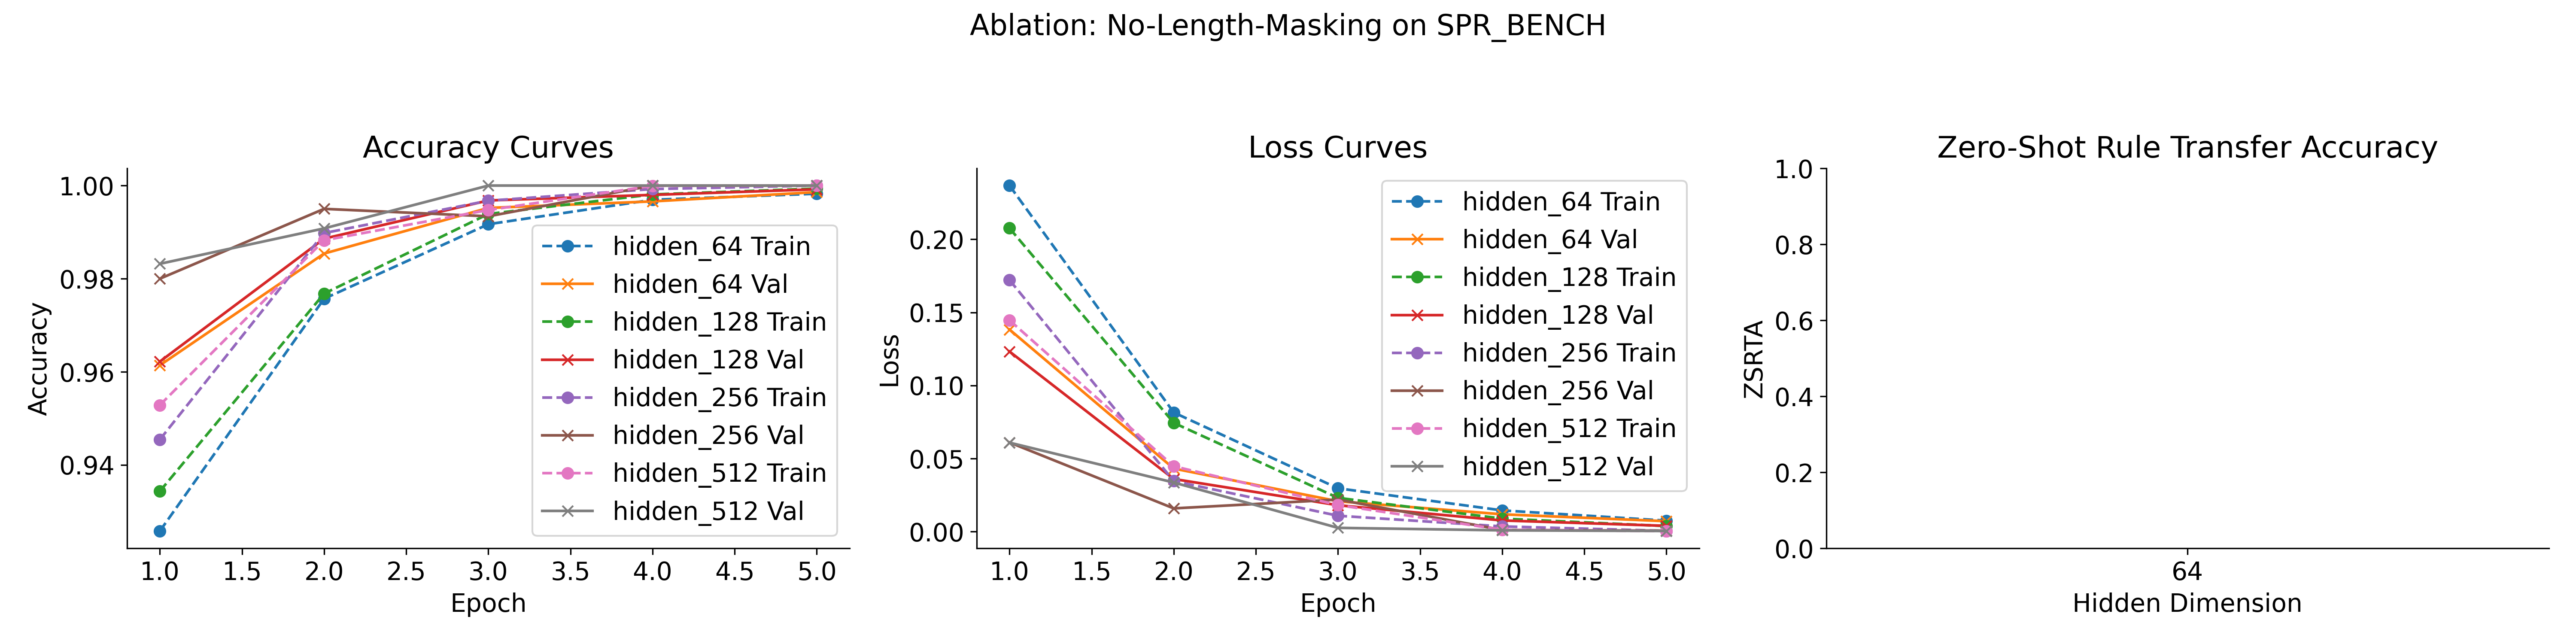
\includegraphics[width=0.75\textwidth]{Ablation_NoLengthMasking.png}
\caption{Ablation study: Training and validation accuracy and loss curves without length masking across different hidden dimensions. The model's performance decreased slightly, indicating the importance of length masking for variable-length sequences. Zero-shot generalization did not improve.}
\label{fig:ablation_no_length_masking}
\end{figure}

\subsection{Multi-Synthetic Dataset Training}

We trained the model on a multi-synthetic dataset that includes a wider variety of rules and sequences to assess the impact of data diversity. As shown in Figure~\ref{fig:ablation_multisynthetic}, increasing the diversity of training data did not improve zero-shot generalization to unseen rules. This suggests that data diversity alone is insufficient to overcome the challenge without explicit mechanisms for rule inference.

\begin{figure}[h!]
\centering
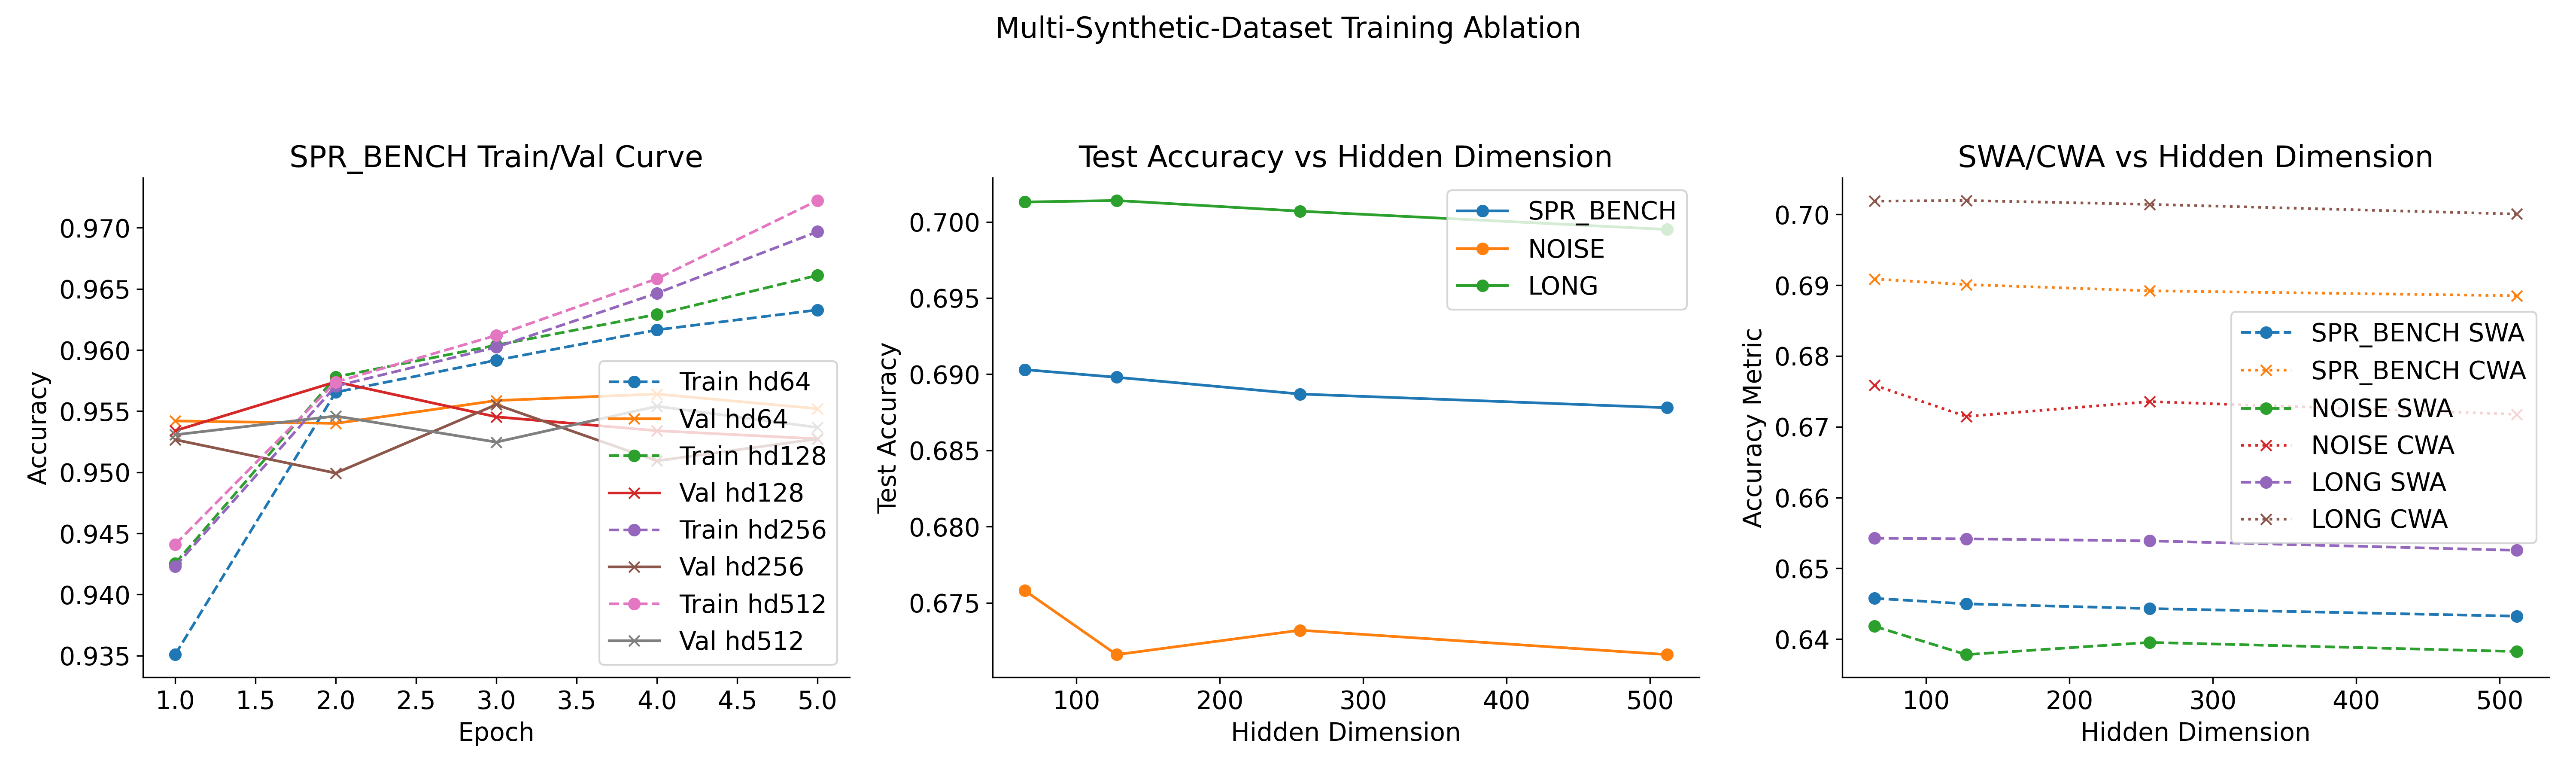
\includegraphics[width=0.75\textwidth]{Ablation_MultiSynthetic_Dataset.png}
\caption{Ablation study: Training and validation accuracy and loss curves when trained on multi-synthetic datasets with increased rule diversity. The model's zero-shot performance did not improve, indicating that additional data diversity does not facilitate generalization to unseen rules.}
\label{fig:ablation_multisynthetic}
\end{figure}

\section{Implementation Details}
\label{sec:implementation_details}

\subsection{Hyperparameters}

We used the following hyperparameters for all experiments unless otherwise specified:

\begin{itemize}
    \item \textbf{Optimizer:} Adam~\citep{goodfellow2016deep}
    \item \textbf{Learning Rate:} $10^{-3}$
    \item \textbf{Batch Size:} 64
    \item \textbf{Number of Epochs:} 5
    \item \textbf{Embedding Dimension:} 128
    \item \textbf{Hidden Dimensions Tested:} 64, 128, 256, 512
    \item \textbf{Sequence Length Handling:} Padding and masking to handle variable-length sequences
\end{itemize}

\subsection{Data Loading}

We utilized the \texttt{datasets} library to load and preprocess the \texttt{SPR\_BENCH} dataset. The following code snippet illustrates the data loading process:

\begin{verbatim}
def load_spr_bench(root: pathlib.Path) -> DatasetDict:
    def _load(split_csv: str):
        return load_dataset(
            "csv",
            data_files=str(root / split_csv),
            split="train",
            cache_dir=".cache_dsets"
        )
    dset = DatasetDict()
    dset["train"] = _load("train.csv")
    dset["dev"] = _load("dev.csv")
    dset["test"] = _load("test.csv")
    return dset
\end{verbatim}

\subsection{Model Definition}

The model was implemented using PyTorch. The key components of the model are defined as follows:

\begin{verbatim}
class SimpleSPRModel(nn.Module):
    def __init__(self, vocab_size, emb_dim, hidden_dim, num_labels):
        super().__init__()
        self.emb = nn.Embedding(vocab_size, emb_dim, padding_idx=0)
        self.gru = nn.GRU(emb_dim, hidden_dim, batch_first=True, bidirectional=True)
        self.lin = nn.Linear(hidden_dim * 2, num_labels)
    def forward(self, x, lengths):
        e = self.emb(x)
        packed = nn.utils.rnn.pack_padded_sequence(
            e, lengths.cpu(), batch_first=True, enforce_sorted=False
        )
        _, h = self.gru(packed)
        h_cat = torch.cat([h[0], h[1]], dim=-1)
        return self.lin(h_cat)
\end{verbatim}

\subsection{Training Procedure}

We trained the model using cross-entropy loss and the Adam optimizer. The training loop included evaluation on the validation set after each epoch to monitor performance. Early stopping was not employed due to the rapid convergence observed.

\end{document}